\chapter{Svolgimento del progetto}
\label{cap:svolgimentodelprogetto}

In questo capitolo descrivo nel dettaglio le attività svolte durante lo \stage,
illustrando le scelte progettuali e le soluzioni adottate per la realizzazione del progetto.
Per i concetti più importanti ho allegato immagini e \snippet{} di codice, per rendere più chiara e comprensibile la spiegazione.
Elenco i principali \textit{framework}, tecnologie ed i \textit{tool} utilizzati per la verifica e la validazione del progetto.

\section{Analisi dei requisiti}
\subsection*{Individuazione dei requisiti}
La prima attività svolta durante lo \textit{stage}, nella prima settimana è stata conosce le persone coninvolte nel progetto e
discutere con loro gli obiettivi e le aspettative del progetto.\\
Successivamente, ho iniziato a studiare i nuvi linguaggi di programmazione e tecnologie che avrei utilizzato durante lo svolgimento delle attività.\\
La seconda settimana invece, ho effettuato l'analisi dei requisiti, attività cruciale condotta 
insieme ai membri del \textit{team}. Con questo processo ho potuto identificarei requisiti 
funzionali, di vincolo e definire i casi d'uso del sistema.

Adottando un approccio in linea con la metodologia agile, ho optato per una raccolta requisiti di tipo incrementale. 
Questo metodo ha permesso una maggiore flessibilità, consentendo aggiornamenti e modifiche dei requisiti in base alle 
mutevoli esigenze del \textit{team} e dell'evoluzione del progetto.

Il primo passo è stato la creazione di un nuovo documento su Confluence. Ho iniziato inserendo le informazioni 
generali del progetto, quali il nome, il \textit{team} coinvolto e una descrizione sintetica. Successivamente, 
ho definito e documentato le convenzioni adottate per la stesura del documento, come la nomenclatura specifica per 
i requisiti e i casi d'uso.

Nella fase successiva, ho proceduto con la stesura effettiva dei requisiti. Inizialmente, ho optato per una 
suddivisione basata sul tipo di requisito, differenziando tra funzionali e di vincolo attraverso due tabelle distinte. 
Tuttavia, nel corso dell'analisi, abbiamo introdotto un ulteriore livello di suddivisione. Questo ci ha permesso di 
classificare i requisiti anche in base al componente del sistema a cui si riferiscono, ovvero \textit{backend}, 
\textit{frontend} e \textit{plugin} Gradle.

Conforme alle aspettative e alla natura agile del progetto, i requisiti sono stati soggetti a continui aggiornamenti 
e modifiche nel corso dello sviluppo. Un esempio significativo è stato l'inserimento dei requisiti facoltativi, 
che inizialmente non erano stati presi in considerazione, ma che si sono rivelati fondamentali per rispondere in 
modo più completo alle esigenze del progetto.

\begin{figure}[!h] 
  \centering 
  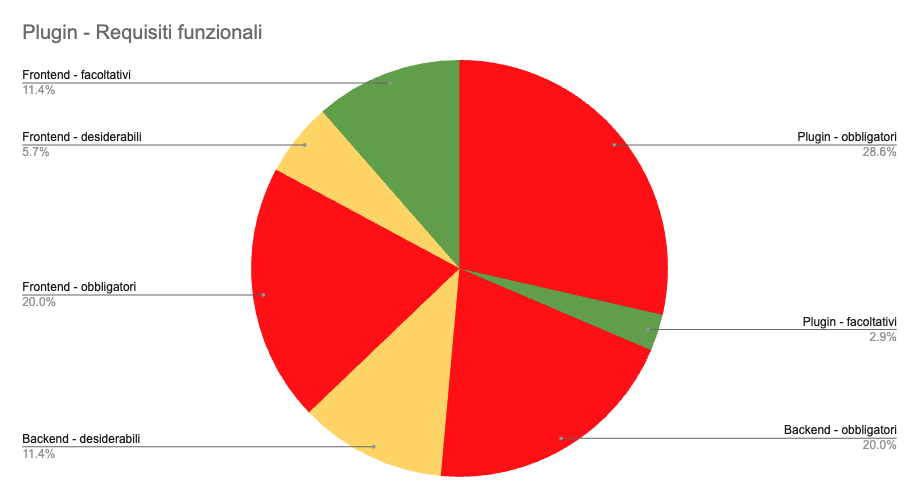
\includegraphics[width=1\columnwidth]{pie-req} 
  \caption{Grafico a torta che mostra la suddivisione in percentuale dei vari requisiti.}
  \label{fig:pie-req}
\end{figure}
\noindent Nella figura \ref*{fig:pie-req} è possibile vedere la suddivisione in percentuale dei requisiti, 
suddivisi come descritto in precedenza.\\
Nella figura \ref*{fig:req-per-importanza} è possibile vedere la suddivisione dei requisiti in base all'importanza.
\begin{figure}[!h] 
  \centering 
  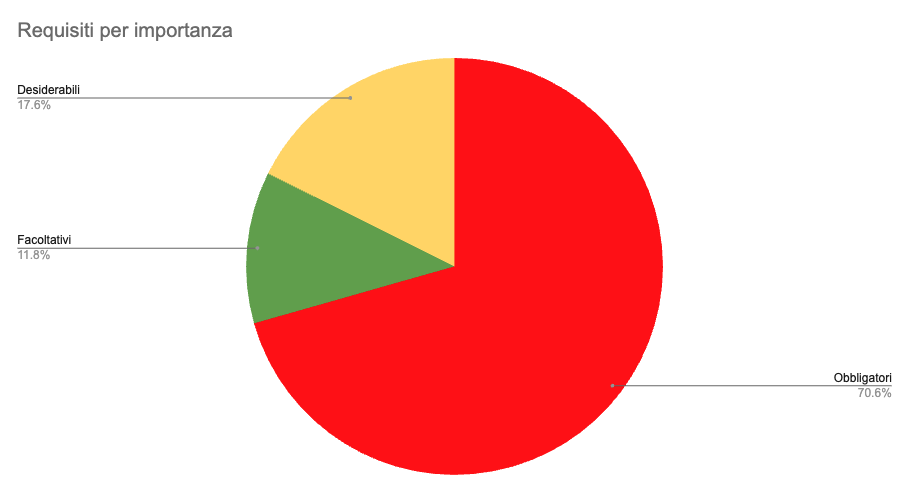
\includegraphics[width=1\columnwidth]{req-per-importanza} 
  \caption{Grafico a torta che mostra la suddivisione dei requisiti in base all'importanza.}
  \label{fig:req-per-importanza}
\end{figure}

\subsection{Tracciamento dei requisiti}
Ad ogni requisito scritto in Confluence ho associato un codice univoco, che mi ha permesso di tracciarlo.
Il codice che ho utilizzato per identificarli è il seguente:
\begin{align*}
  \textbf{R[F/V]-[O/D]-[B/F/P]-[001]}
\end{align*}
Nello specifico:
\begin{itemize}
    \item \textbf{RF}: requisito funzionale, \textbf{RV}: requisito di vincolo;
    \item \textbf{O}: obbligatorio, \textbf{D}: desiderabile, \textbf{F}: facoltativo;
    \item \textbf{P}: componente del sistema a cui si riferisce, \textbf{B}: \textit{backend}, \textbf{F}: \textit{frontend}, \textbf{P}: \textit{plugin} Gradle;
    \item \textbf{001}: numero progressivo del requisito.
\end{itemize}

\noindent Per il tracciamento dei requisiti, ho utilizzato un metodo efficace utilizzando Confluence e Jira. 
Nella tabella dei requisiti, che ho creato su Confluence e identificabile tramite la figura \ref*{fig:jira-confluence-requisiti}, 
ho inserito una nuova colonna. In questa colonna, ho inserito il riferimento alla \textit{issue} di 
Jira corrispondente a ciascun requisito.\\
Questa integrazione tra Confluence e Jira ha permesso di collegare direttamente ogni requisito a una specifica 
\textit{issue} di Jira, che ne dettaglia l'implementazione. Grazie a questo collegamento, ho ottenuto una visione più 
completa e dettagliata del progetto, migliorando notevolmente la precisione nel tracciamento dei requisiti.\\
Inoltre, ho sfruttato la funzionalità di visualizzazione automatica in modalità \textit{read-only} su Confluence. 
Questo ha permesso di consultare direttamente nella tabella dei requisiti le informazioni essenziali relative alle \textit{issues} 
di Jira, come lo stato di avanzamento e le descrizioni dettagliate, quando necessario.

Ogni \textit{issue} l'ho collegata ad un'epica, che rappresenta un insieme di \textit{issues} correlate tra loro. In tutto ho creato 4 epiche,
una per ogni componente del progetto (\textit{backend}, \textit{frontend}, \textit{plugin} Gradle e analisi).\\
\begin{figure}[!h] 
  \centering 
  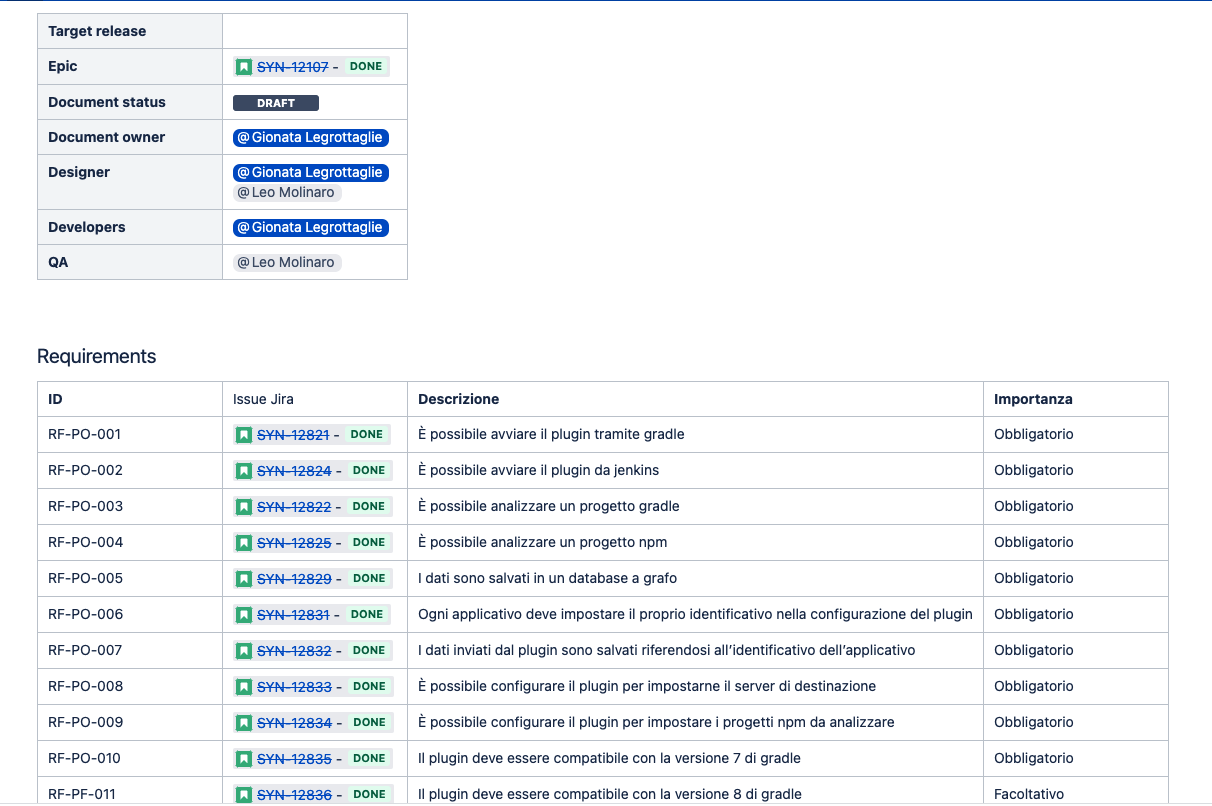
\includegraphics[width=.9\columnwidth]{jira-confluence-requisiti} 
  \caption{Tabella che mostra il tracciamento dei requisiti su Confluence, con il collegamento a Jira.}
  \label{fig:jira-confluence-requisiti}
\end{figure}

Tramite Jira ho creato un \textit{board} per il progetto, che mi ha permesso di visualizzare in modo chiaro e 
semplice lo stato di avanzamento del progetto, vedi la figura \ref*{fig:board-jira}.
All'interno di questa \textit{board} è possibile visualizzare, per ogni \textit{record} della tabella, il tipo di \textit{issue}, il vodice, la priorità, lo stato,
la persona assegnata, la stima in giorni/ore e, per l'intero \textit{sprint}, la stima totale in giorni/ore.\\


\begin{figure}[!h] 
  \centering 
  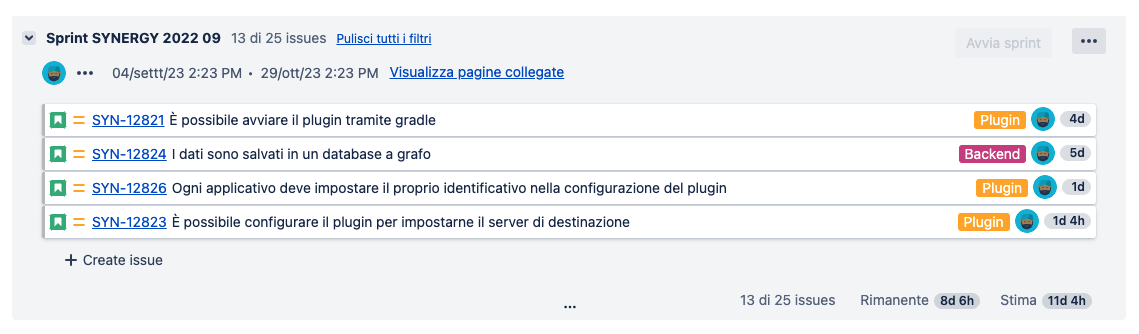
\includegraphics[width=1\columnwidth]{board-jira} 
  \caption{\textit{Board} di Jira che mostra lo stato di avanzamento del progetto.}
  \label{fig:board-jira}
\end{figure}

\noindent Jira offre una gamma di funzionalità avanzate, tra cui spicca la capacità di creare dei \textit{plan}. 
Questa funzionalità si rivela particolarmente utile nella pianificazione delle \textit{issues}, consentendo di organizzarle 
efficacemente in base alle loro date di inizio e fine, permettendoti di avere una visualizzazione grafica del 
progetto attraverso un grafico di \textit{gantt}. \\ Questo grafico rappresenta visivamente le \textit{issues} 
in relazione alle loro date di inizio e fine, offrendo una panoramica chiara e immediata dello stato di avanzamento del progetto, mettendo
in risalto anche le \textit{milestone} prefissate nel piano di lavoro.\\ 
Inoltre, una funzionalità di Jira permette di modificare e riallocare le \textit{issues} con facilità, 
adattandosi dinamicamente alle esigenze del progetto in corso.


\section{Progettazione architetturale}
\subsection*{Progettazione delle strutture dati}
La prima fase della progettazione architetturale è stata la progettazione delle strutture dati. 
Era molto importante progettare le strutture dati in modo da poterle utilizzare in modo efficiente e 
veloce, in quanto il progetto si basa su di esse.\\
L'obiettivo era quello di creare una struttura dati che permettesse di rappresentare un grafo di dipendenze tra i vari pacchetti di un progetto.\\
Ogni nodo del grafo rappresenta un pacchetto, ed aveva bisogno di avere le seguenti informazioni:
\begin{itemize}
  \item \textbf{id}: identificativo univoco del nodo;
  \item \textbf{\textit{group}}: nome del gruppo del pacchetto;
  \item \textbf{\textit{name}}: nome del pacchetto;
  \item \textbf{\textit{version}}: versione del pacchetto;
  \item \textbf{tipo}: tipo del pacchetto, può essere Java o JavaScript;
\end{itemize}

\noindent Ogni arco del grafo, come mostrato in figura \ref*{fig:esempio1-neo4j} rappresenta una dipendenza tra due pacchetti, 
ed ha bisogno di avere le seguenti informazioni:
\begin{itemize}
  \item \textbf{id}: identificativo univoco dell'arco;
  \item \textbf{from}: identificativo del nodo di partenza;
  \item \textbf{to}: identificativo del nodo di arrivo;
  \item \textbf{require}: numero di versione richiesto dal pacchetto di partenza;
  \item \textbf{variants}: rappresenta la lista di utilizzi del pacchetto, es: \textit{compileOnly, implementation, testImplementation}; 
\end{itemize}

\begin{figure}[!h] 
  \centering 
  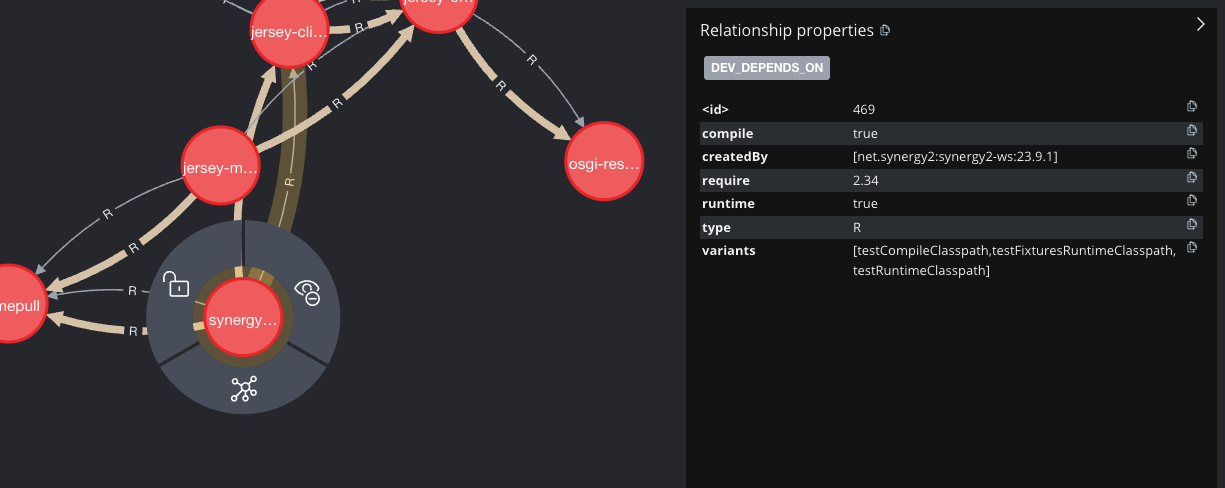
\includegraphics[width=1\columnwidth]{esempio1-neo4j} 
  \caption{Esempio di grafo di dipendenze tra pacchetti.}
  \label{fig:esempio1-neo4j}
\end{figure}

Prima di arrivare alla struttura finale, abbiamo fatto diverse prove, cercando di trovare la struttura più adatta alle nostre esigenze.\\
La versione finale, come mostrato in figura \ref{fig:struttura-grafo} ha saputo soddisfare tutte le nostre esigenze.\\
Da ogni nodo possono partire tre tipi di archi, ognuno con una funzione diversa; Il primo tipo di arco è quello che rappresenta 
una dipendenza diretta tra due pacchetti, quindi ad esempio se il pacchetto \textbf{A 1.0} dipende dal pacchetto \textbf{B 1.0 }, 
allora dal nodo A parte un arco, nella figura è rappresentato con una linea continua, che punta al nodo B.\\
Il secondo tipo di arco è quello che rappresenta una dipendenza transitiva tra due pacchetti, quindi ad esempio se il pacchetto
\textbf{A 1.0} dipende dal pacchetto \textbf{C 1.0} e il pacchetto \textbf{C 1.0} dipende dal pacchetto \textbf{D 3.0},
allora dal nodo A parte un arco, nella figura è rappresentato con una linea tratteggiata, che punta al nodo \textbf{D 3.0}.\\
Il terzo ed ultimo tipo di arco è quello che rappresenta una dipendenza transitiva tra due pacchetti, ma con una versione diversa,
quindi ad esempio se il pacchetto \textbf{A 1.0} dipende dal pacchetto \textbf{B 1.0} e il pacchetto \textbf{B 1.0} dipende dal pacchetto 
\textbf{D 2.0}, ma il pacchetto \textbf{A 1.0} dipende anche, in modo diretto o transitivo, dal pacchetto \textbf{D 3.0}, 
allora dal nodo \textbf{B 1.0} parte un arco, nella figura è rappresentato con una linea tratteggiata, a tratto più piccolo, 
che punta al nodo \textbf{D 3.0}.\\
Questo ultimo tipo di arco l'abbiamo introdotto per poter gestire le dipendenze transitiva con versioni diverse, dato che al rilascio di un
pacchetto finale da installare, la versione che verrà installata sarà quella più recente, quindi in questo caso la versione \textbf{D 3.0}.\\

\begin{figure}[!h] 
  \centering 
  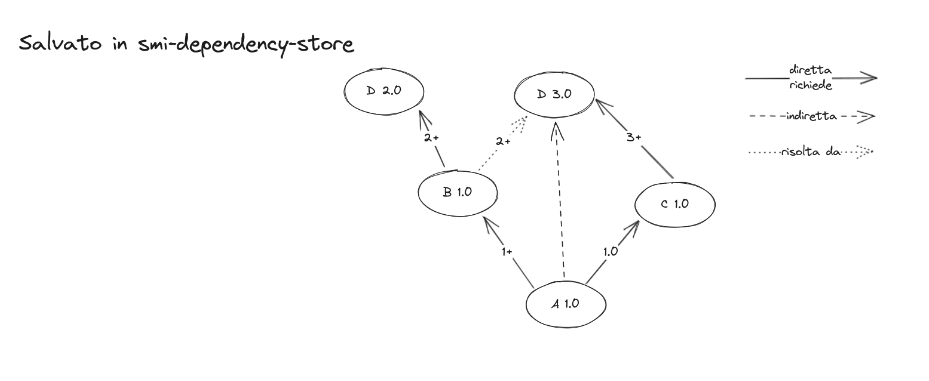
\includegraphics[width=1\columnwidth]{struttura-grafo} 
  \caption{Struttura finale del grafo di dipendenze.}
  \label{fig:struttura-grafo}
\end{figure}

\subsection*{Progettazione \textit{plugin} di analisi delle dipendenze}

Il progetto Java per la creazione del \textit{plugin} Gradle, smi-dependency-analyzer, è stato sviluppato utilizzando il \textit{framework} Gradle.\\
Gradle mette a disposizione delle \textit{API} per la creazione di \textit{plugin} personalizzati,
che permettono di estendere le funzionalità del \textit{build tool}.\\
Il progetto contiene tre \textit{package} principali:
\begin{itemize}
  \item \textbf{\textit{model}}: contiene le classi che rappresentano le strutture dati utilizzate dal \textit{plugin};
  \item \textbf{\textit{logic}}: contiene le classi che rappresentano la logica del \textit{plugin}, dove vengono eseguite le operazioni di analisi, 
  trasformazione e trasferimento dei dati;
  \item \textbf{task}: contiene le classi che rappresentano i \textit{task} del \textit{plugin}, ovvero le operazioni che possono essere eseguite dal \textit{plugin} 
  e la classe di registrazione del \textit{plugin}.
\end{itemize}

Ho definito anche una classe che rappresenta l'oggetto di configurazione del \textit{plugin}, 
che contiene le informazioni necessarie per l'esecuzione del \textit{plugin} e per il salvataggio dei dati, un esempio lo si può visualizzare nello \snippet{} \ref*{lst:plugin-config}

\begin{lstlisting}[
  language=Groovy, 
  caption={Esempio di configurazione del \textit{plugin} Gradle, utilizzando il linguaggio Groovy.},
  captionpos=b, 
  label={lst:plugin-config}
  ]
  smi_dependency_analyzer {
    username = "nome_utente"
    password = "private_key"
    url = "http://localhost:8080/smi-dependency-store"
    npmProject {
        packageJson = "/projects/esempio1/client/package.json"
        packageLockJson = "/projects/esempio1/client/package-lock.json"
    }
  }
\end{lstlisting}

L'idea di base del \textit{plugin} è quella di creare un \textit{task} che avvii il task standard messo a disposizione da Gradle
per la creazione del \textit{dependency tree}, ovvero \textit{dependencyInsight}, e con l'output di questo task,
creare un grafo di dipendenze, che verrà inviato al \textit{server} per essere salvato.\\
Per i proggetti Npm invece, il \textit{plugin} legge il file \textit{package-lock.json}. Questo file viene generato automaticamente
da Npm e contiene tutte le informazioni necessarie per la creazione del grafo di dipendenze.\\
Un prerequisito per il funzionamento del \textit{plugin} è che sia stato eseguito il comando \textbf{\textit{npm install}},
in modo da avere tutte le dipendenze installate nella cartella \textit{node\_modules} e quindi avere il file \textit{package-lock.json}.

Una volta raccolte tutte le informazioni necessario, effettuo una chiamata \textit{REST} di tipo \textit{PUT} al \textit{server},
per salvare il grafo di dipendenze.\\
\subsection*{Progettazione \textit{backend}}
Il progetto del \textit{backend}, denominato \textbf{smi-dependency-store}, l'ho suddiviso in quattro \textit{package} principali:
\begin{itemize}
  \item \textbf{model}: contiene le classi che rappresentano le strutture dati utilizzate dal \textit{server} e 
  le classi di configurazione;
  \item \textbf{dao}: contiene le classi utilizzate per la comunicazione con il \textit{database}, ed in questo caso
  conteneva la classe \textbf{PackageNodeDao} che gestiva l'inserimento/aggiornamento/cancellazione dell'entità nodo \textbf{PackageNode}
  e la classe \textbf{DependencyLinkDao} che gestiva l'inserimento/aggiornamento/cancellazione dell'entità arco \textbf{DependencyLink};
  \item \textbf{logic}: contiene le classi che rappresentano la logica del \textit{server}, dove vengono eseguite le operazioni di analisi, 
  trasformazione e chiamate alle classi \textit{dao};
  \item \textbf{rest}: contiene le classi che rappresentano i \textit{controller} del \textit{server}, 
  ovvero tutti i servizi \textit{REST} messi a disposizione dal \textit{server}.
\end{itemize}

Per la configurazione del \textit{server}, ho previsto quattro diversi file di configurazione, uno per ogni funzionalità del \textit{server}:
\begin{itemize}
  \item \textbf{neo4j.yml}: contiene le informazioni per la connessione al \textit{database} Neo4j, come l'indirizzo, l'username e la password. Vedi snippet \ref*{lst:neo4j-config};
  \begin{lstlisting}[
    caption={Esempio di configurazione del \textit{neo4j.yml}}
    captionpos=b, 
    label={lst:neo4j-config}
    ]
  url: "bolt://localhost:7689"
  username: "neo4j"
  password: "neo4jlocal"
  \end{lstlisting}
  \item \textbf{token.yml} contiene le informazioni per la generazione del \textit{token}, come la chiave segreta, il \textit{clientId}, il \textit{clientSecret}, il
    nome del \textit{server} e la durata del \textit{token}. Vedi snippet \ref*{lst:token-config}.
    Questo vuol dire che se non configurato l'\textit{LDAP}, ci sarà un solo utente che potrà accedere al \textit{server}, 
    utilizzando come \textit{username} e \textit{password} quelle configurate come \textit{clientId} e \textit{clientSecret}.\\
    Il token \textit{JWT} generato avrà una durata di 30 minuti e sarà firmato con la chiave segreta \textit{SECRET\_KEY}.
    \begin{lstlisting}[caption={Esempio di configurazione del \textit{token.yml}.},captionpos=b, label={lst:token-config}]
  hmacSha512Key: "SECRET_KEY"
  clientId: "admin"
  clientSecret: "admin"
  issuer: "dependency_store"
  validity: 1800000
    \end{lstlisting}
  \item \textbf{logger.yml}: contiene le informazioni per la configurazione del \textit{logger}, come il livello di log, il formato del \textit{log} e il file di output. Vedi snippet \ref*{lst:logger-config}.
    Questa configurazione viene passata ad una libreria sviluppata da \azienda{}, che è un \textit{wrapper} della libreria \textit{slf4j}, nota libreria per la gestione dei \textit{log} in Java.
    Il campo \textit{params} contiene le informazioni per la configurazione del livello di \textit{log} per ogni \textit{package} del \textit{server}. 
    Questo mi permette di avere un livello di \textit{log} diverso per ogni \textit{package} del \textit{server}, molto utile per il \textit{debug}.
    \begin{lstlisting}[caption={Esempio di configurazione del \textit{logger.yml}.},captionpos=b, label={lst:logger-config}]
defaultLogLevel: "info"
showDateTime: true
dateTimeFormat: "yyyy-MM-dd HH:mm:ss"
showThreadName: false
showShortLogName: true
logFile: "../logs/out.log"
  params:
   com.smi: "debug"
  \end{lstlisting}
 \item \textbf{ldap.yml} contiene le informazioni per la configurazione dell'\textit{LDAP}, come l'indirizzo del \textit{server}, 
 il dominio ed un \textit{flag} che indica se utilizzare una connessione sicura o meno. Vedi snippet \ref*{lst:ldap-config}.
  \begin{lstlisting}[caption={Esempio di configurazione dell'\textit{ldap.yml}.},captionpos=b, label={lst:ldap-config}]
  url: "ldap://10.10.99.1"
  domain: "DOMIONIO_AZIENDA"
  ssl: false
  \end{lstlisting}
\end{itemize}

Nel corso dello sviluppo, ho adottato il \textit{design pattern Singleton} per l'implementazione delle classi Java 
dedicate alla logica, \textit{dao} e configurazione. Questo approccio assicura che esista una sola istanza di queste classi 
all'interno del \textit{server}, utilizzata condivisamente da tutte le altre classi.

Per realizzare il \textit{Singleton} in Java, ho sfruttato una libreria sviluppata da \azienda{}, che facilita 
l'implementazione di questo pattern in modo efficiente e rapido. L'\textit{snippet} \ref*{lst:esempio-singleton} mostra un esempio 
di questa implementazione per la classe \textbf{PackageNodeDao}. Abbiamo optato per l'uso di una \textit{inner class} statica, 
dotata di un campo statico \textbf{SingletonHolder}. Quest'ultimo contiene un metodo \textit{get} che accetta una \textit{lambda expression}, 
restituendo un oggetto di tipo \textbf{PackageNodeDao}. Questa strategia garantisce la creazione dell'istanza solo all'occorrenza, 
evitando la creazione anticipata al momento del caricamento della classe e assicurando l'unicità dell'istanza anche in contesti di \textit{multithreading}.

La classe \textbf{SingletonHolder} non solo gestisce la creazione dell'istanza, ma offre anche la possibilità di personalizzare i metodi 
di \textbf{PackageNodeDao}. Se si desidera modificare i metodi di questa classe, è possibile definire una sottoclasse di \textbf{PackageNodeDao}, 
nominata \textbf{PackageNodeDaoPers}. In questo caso, grazie all'uso della \gls{reflection} di Java, 
il \textbf{SingletonHolder} restituirà automaticamente un'istanza di \textbf{PackageNodeDaoPers}, permettendo una personalizzazione avanzata.


\begin{lstlisting}[
  language=Java, 
  caption={Esempio di implementazione del \textit{design pattern} Singleton in Java.},
  captionpos=b, 
  label={lst:esempio-singleton}
  ]
  public class PackageNodeDao {
    protected PackageNodeDao () { }
    public static PackageNodeDao get() {
      return Singleton.INSTANCE.get(PackageNodeDao::new);
    }
    private static class Singleton {
        private static final SingletonHolder<PackageNodeDao> INSTANCE = new SingletonHolder<> (PackageNodeDao.class);
    }
  }
\end{lstlisting}

\subsection*{Progettazione \textit{frontend}}

Per la progettazione del \textit{frontend} siamo dal \textit{mockup} grafico realizzato in fase di analisi.
Questo ci ha permesso di avere una visione chiara e dettagliata dell'interfaccia grafica, 
semplificando notevolmente la fase di sviluppo.\\
Il \textit{mockup} è stato realizzato utilizzando il \textit{tool} gratuito \textit{online} \textit{excalidraw}, che permette di creare grafiche semplici
come quella mostrata in figura \ref*{fig:mockup}.\\
\begin{figure}[!h] 
  \centering 
  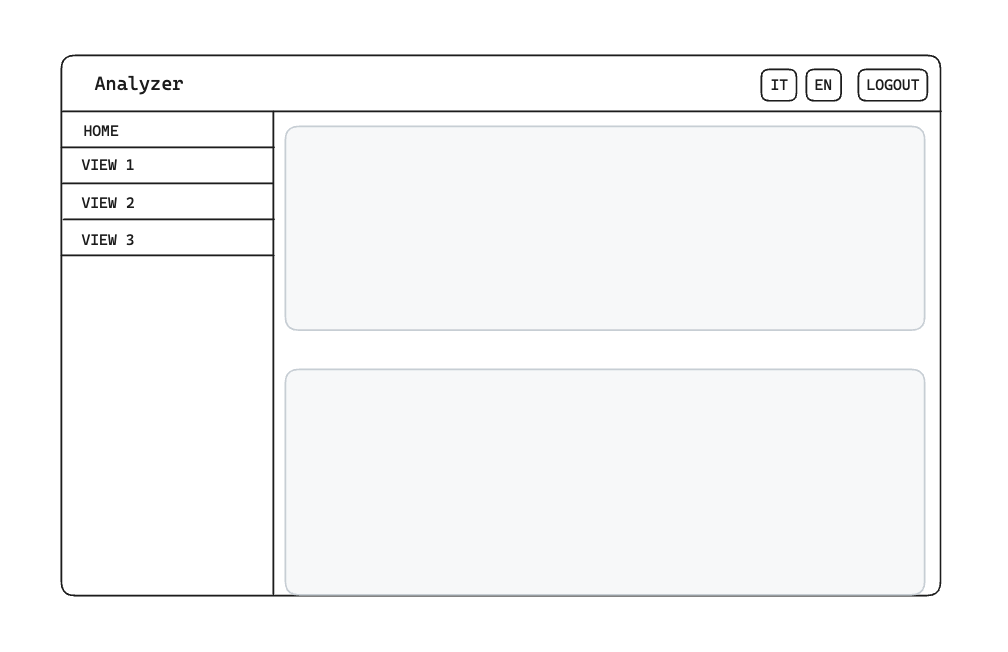
\includegraphics[width=1\columnwidth]{mockup} 
  \caption{\textit{Mockup} grafico dell'interfaccia grafica.}
  \label{fig:mockup}
\end{figure}

Da qui ho iniziato a sviluppare il \textit{frontend}, utilizzando il \textit{framework} Angular.\\
Per prima cosa creato le due cartelle principali del progetto, la prima ,\textbf{commons}, contiene i componenti, i servizi e i modelli che possono 
essere utilizzati in più componenti;
la seconda, \textbf{features}, contiene a sua volta una cartella per ogni funzionalità del \textit{frontend}.
Ho creato quindi le cartelle \textit{home}, \textit{login}, \textit{query} e \textit{find-by-project}. 
  Ogni cartella al suo interno contiene i componenti, i servizi e i modelli relativi alla funzionalità. 
  Nella figura \ref*{fig:frontend-structure} è possibile vedere la struttura del progetto.
  \begin{figure}[!h] 
    \centering
    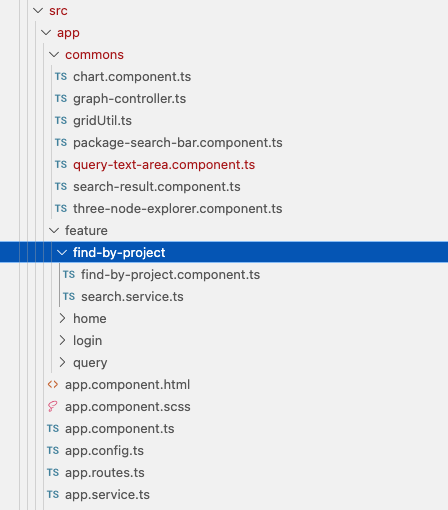
\includegraphics[width=.5\columnwidth]{frontend-structure} 
    \caption{Struttura del progetto \textit{frontend}.}
    \label{fig:frontend-structure}
  \end{figure}  

Per la scrittura del codice ho seguito le linee guida di Angular, rilasciate nel loro sito ufficiale \cite{site:angular-style-guide}.\\

Come mostrato in figura \ref*{fig:frontend-1}, l'interfaccia grafica è formata da una barra di navigazione, che contiene il nome del progetto,
il pulsante per il \textit{logout} ed i pulsanti per cambiare la lingua dell'interfaccia grafica.\\
Sotto la barra di navigazione è presente una \textit{sidebar}, che contiene i pulsanti per accedere alle varie funzionalità del \textit{frontend} 
ed il contenitore principale che mostra il contenuto della funzionalità selezionata.\\
\begin{figure}[h]
  \centering
  \begin{minipage}{0.45\textwidth}
      \centering
      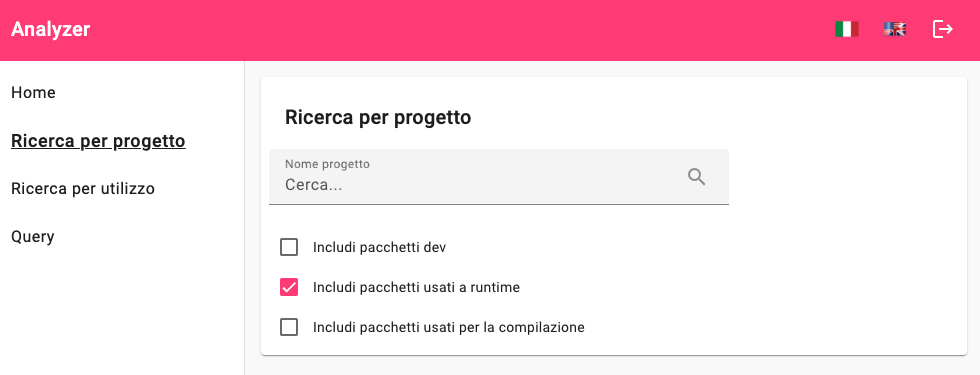
\includegraphics[width=\textwidth]{frontend-1}
      \caption{Modulo di ricerca dipendenze per progetto.}
      \label{fig:frontend-1}
  \end{minipage}\hfill
  \begin{minipage}{0.45\textwidth}
      \centering
      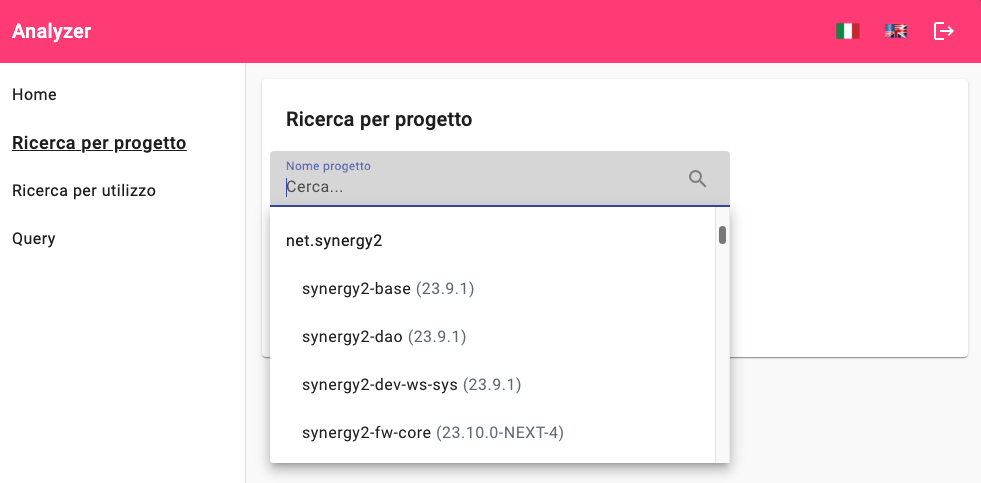
\includegraphics[width=\textwidth]{frontend-2}
      \caption{Casella di ricerca con lista di suggerimenti.}
      \label{fig:frontend-2}
  \end{minipage}
\end{figure}
Le voci di menu presenti nella \textit{sidebar}, oltre alla funzionalità \textit{home}, sono tre:
\begin{itemize}
  \item \textbf{Ricerca per progetto}: Come mostrato in figura \ref*{fig:frontend-1}, in questo modulo, tramite la barra di ricerca
   è possibile inserire il nome completo, formato da \textit{group}, \textit{name} e \textit{version}, di un pacchetto e visualizzare
    le informazioni relative a quel pacchetto.\\
    Tuttavia per rendere più semplice la ricerca, ho aggiunto una funzionalità di suggerimento, che mostra la lista di pacchetti conosciuti dal 
    \textit{server}, che iniziano con la stringa inserita nella barra di ricerca e raggruppati per \textit{group}, come rappresentato in figura \ref*{fig:frontend-2}.\\
    Sotto alla casella di testo sono presenti tre \textit{checkbox}, che permette di scegliere se includere i pacchetti targati come \textit{dev}, 
    se invcudere i pacchetti utilizzati solo durante la compilazione dei progetti o se includere tutti i pacchetti utilizzati a runtime
    da un progetto.\\
    Una volta avviata la ricerca, viene mostrato il risultato sotto di esso, come mostrato in figura \ref*{fig:frontend-3}.\\
    Qui troviamo tre possibili visualizzazioni del risultato: a grafo, ad albero e a lista.\\
    Nella visualizzazione tabellare abbiamo una lista piatta di tutti i pacchetti, con le informazioni principali, trascurando i collegamenti tra i pacchetti.\\
    Questa visualizzazione può tornare utile quando si vuole avere una visione d'insieme di tutti i pacchetti utilizzati da un progetto.\\
    Nella visualizzazione ad albero invece, abbiamo una visualizzazione gerarchica dei pacchetti, dove ogni nodo rappresenta un pacchetto ed espanendo un nodo
    è possibile vedere i pacchetti da cui dipende.\\
    In questo modo riusciamo a capire a come mai un pacchetto è stato incluso nel progetto, e quali altri pacchetti sono stati inclusi a causa di esso.\\
    Nella visualizzazione a grafo invece, abbiamo una visualizzazione grafica dei pacchetti, dove ogni nodo rappresenta un pacchetto e gli archi rappresentano
    le dipendenze tra i pacchetti.\\
    \begin{figure}[h]
      \centering
      \begin{minipage}{0.60\textwidth}
          \centering
          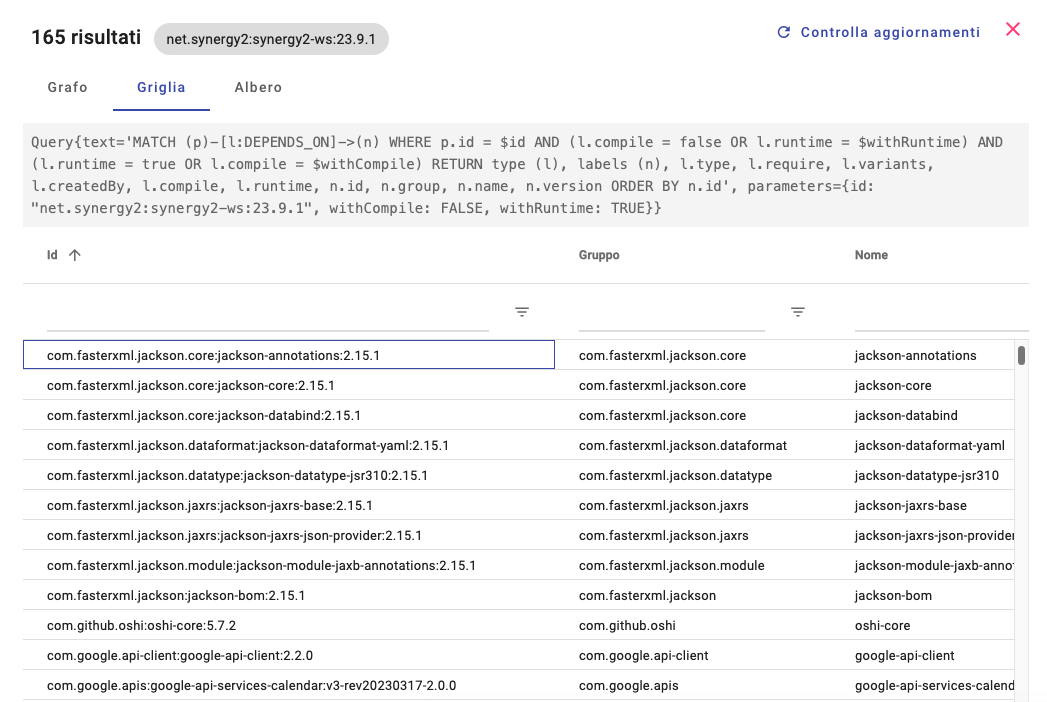
\includegraphics[width=\textwidth]{frontend-3.png} 
          \caption{Risultato tabellare.}
          \label{fig:frontend-3}
      \end{minipage}\hfill
      \begin{minipage}{0.30\textwidth}
          \centering
          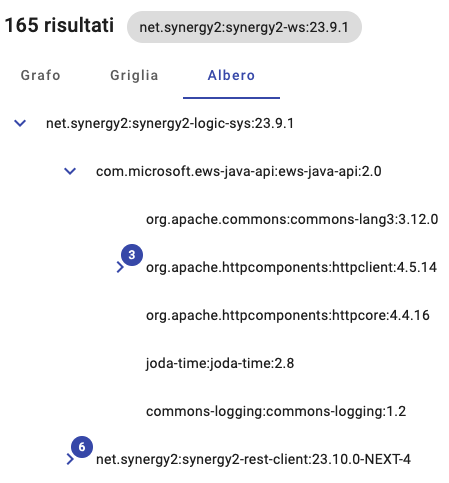
\includegraphics[width=\textwidth]{frontend-4.png} 
          \caption{Risultato ad albero.}
          \label{fig:frontend-4}
      \end{minipage}
    \end{figure}
    Inoltre, in visualizzazione è possibile fare un controllo sulla presenza di aggiornamenti e vulnerabilità, ad esempio, come mostrato in figura \ref*{fig:frontend-8},
    vengono mostrati tutti i pacchetti che hanno una versione più recente di quella utilizzata dal progetto.\\
    \begin{figure}[!h] 
      \centering
      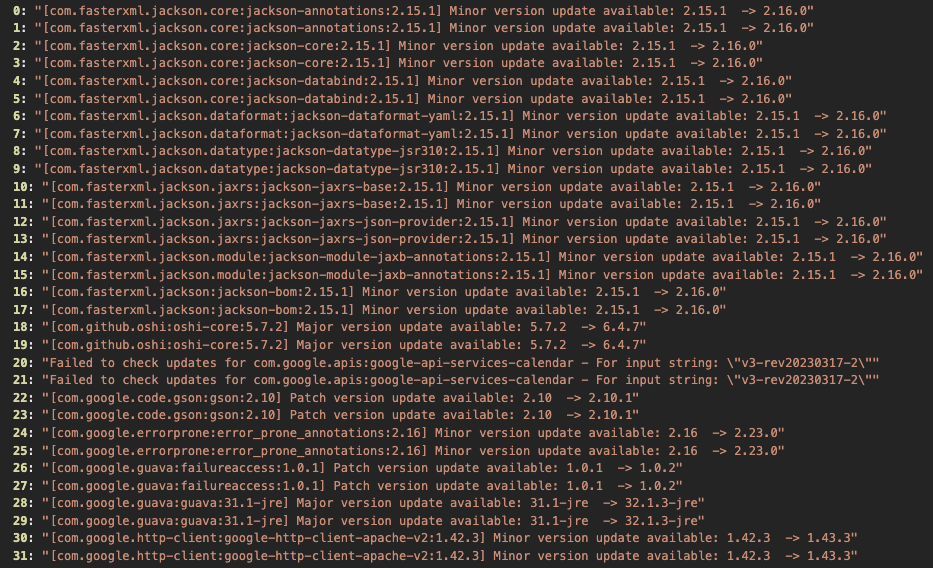
\includegraphics[width=.7\columnwidth]{frontend-8.png} 
      \caption{Visualizzazione di tutti gli aggiornamenti disponibili.}
      \label{fig:frontend-8}
    \end{figure}  
  \item \textbf{Ricerca per utilizzo}: La ricerca avviene in modo simile a quella per progetto, ma in questo caso, il risultato mostra solo una 
  griglia con i pacchetti che utilizzano il pacchetto cercato.\\
  Nell'esempio in figura \ref*{fig:frontend-5}, ho cercato il pacchetto \textbf{net.synergy2:synergy2-base:23.9.1}, e il risultato mostra tutti i pacchetti che lo utilizzano.\\
  Oltre alla griglia, è presente anche un \textit{box} che mostra la \textit{query}, con la sintassi Cypher, utilizzata per la ricerca.\\


  \begin{figure}[!h] 
    \centering
    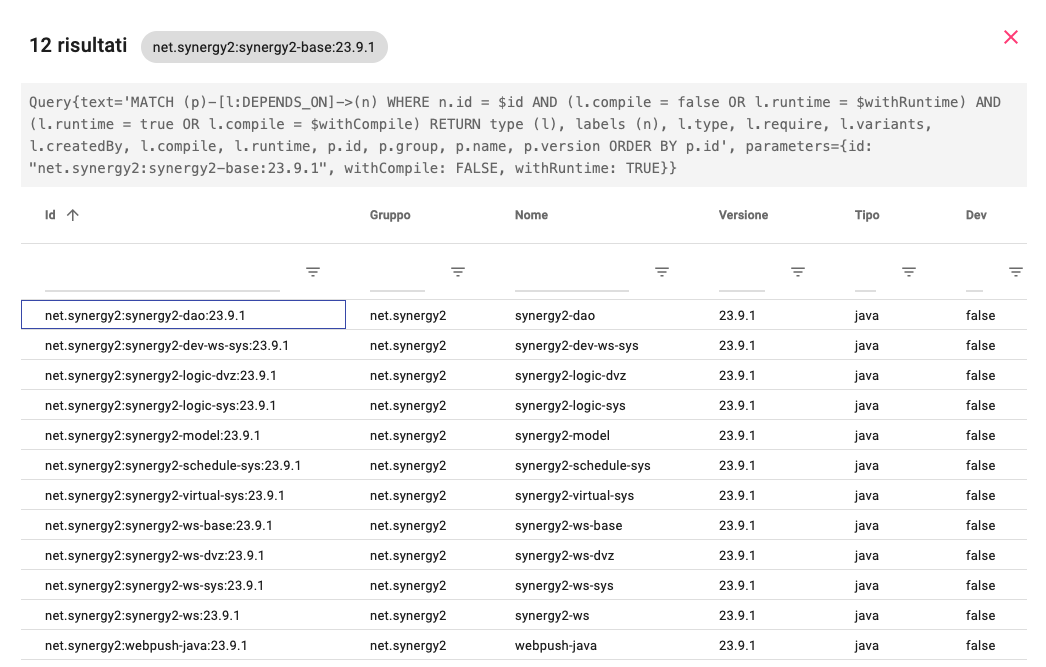
\includegraphics[width=.9\columnwidth]{frontend-5.png} 
    \caption{Esempio di ricerca per utilizzo.}
    \label{fig:frontend-5}
  \end{figure}  
  \item \textbf{\textit{Query}}: in quest'ultima funzionalità, come mostrato in figura \ref*{fig:frontend-5}, è possibile inserire una \textit{query} Cypher libera e visualizzare il risultato in 
  formato \textit{JSON}. Questo può tornare utile quando si vuole effettuare una ricerca più complessa, che non è possibile effettuare con le altre funzionalità.\\
  \begin{figure}[!h] 
    \centering
    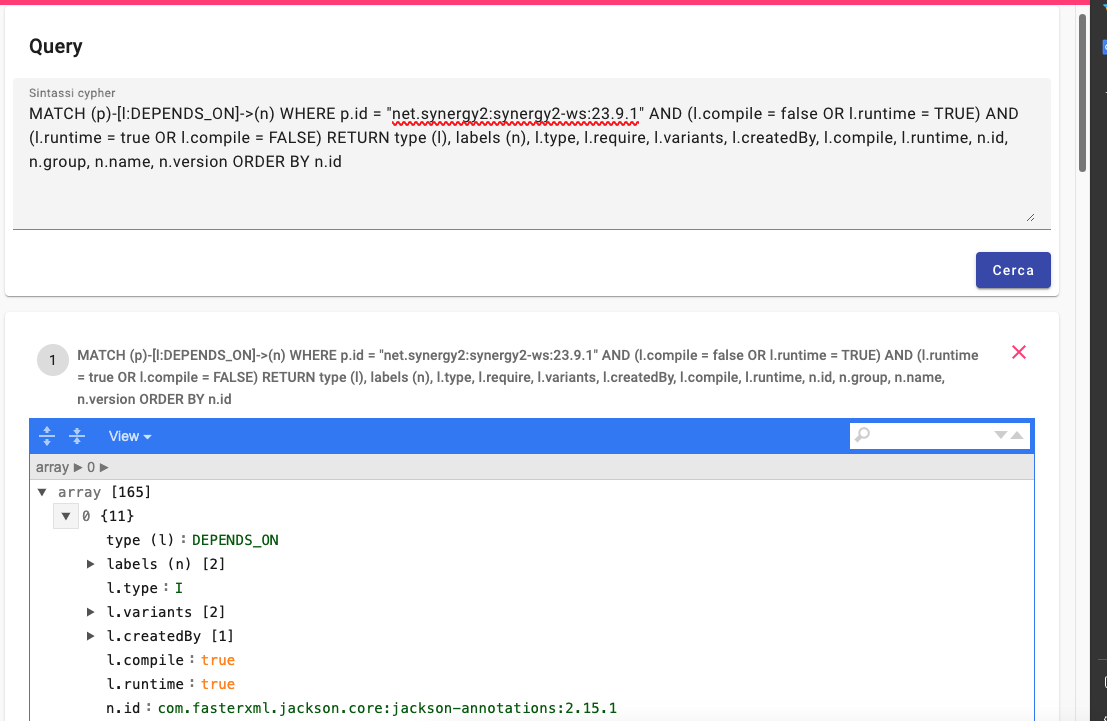
\includegraphics[width=.9\columnwidth]{frontend-6.png} 
    \caption{Modalità \textit{query} libera.}
    \label{fig:frontend-6}
  \end{figure}  

\end{itemize}


\section*{Codifica}
\subsection*{Librerie e \textit{framework} utilizzati}
\subsubsection*{Jersey}
Per la creazione servizi \textit{REST}, ho utilizzato Jersey, che tramite annotazioni su metodi e classi, 
mi ha permesso di creare facilmente i vari servizi.
Lo \snippet{}  \ref*{lst:rest-service} mostra un esempio di \textit{servizio REST} che restituisce tutte le dipendenze di un pacchetto.\\
\begin{lstlisting}[language=Java, caption={Esempio di \textit{servizio REST} utilizzando Jersey.},captionpos=b, label={lst:rest-service}]
  @GET ()
  @Path ("dependency/byPackage/{id}")
  @Produces (MediaType.APPLICATION_JSON) @Consumes (MediaType.APPLICATION_JSON)
  public Response byPackage (@PathParam ("id") String id, 
        @QueryParam ("withDev") boolean withDev, 
        @QueryParam ("withCompile") boolean withCompile, 
        @QueryParam ("withRuntime") boolean withRuntime
  ) {
      return Response.ok (DependencyLogic.get ().getDependenciesByPackage (id, withDev, withCompile, withRuntime)).build ();
  }
\end{lstlisting}

\subsubsection*{Neo4j}
Per la gestione del \textit{database} Neo4j, ho utilizzato la libreria \textbf{Neo4j Java Driver}, 
che mette a disposizione una serie di classi e metodi per l'apertura e la gestione delle connessioni al \textit{database} e 
per l'esecuzione di \textit{query} Cypher.\\

\subsubsection*{Smi-commons}
Per la gestione delle operazioni comuni, come la gestione del \textit{logger}, la gestione delle eccezioni, la lettura dei 
file di configurazione e la gestione del \textit{token}, ho utilizzato una libreria sviluppata da \azienda{}, denominata \textit{smi-commons}.\\

\subsubsection*{Nx}
Per la creazione e gestione del progetto Angular, ho utilizzato il \textit{tool} \textbf{Nx}, 
che permette di creare progetti Angular senza dover pensare alla struttura del progetto.\\
Nx mette a disposizione una serie di comandi per la creazione di progetti, moduli, componenti, servizi e librerie,
e permette di eseguire i \textit{test} e il \textit{build} del progetto.\\
Nx viene utilizzato principalmente per la gestione di progetti \textit{monorepo}, ovvero progetti che contengono più applicazioni,
in modo da poter condividere le librerie tra le varie applicazioni.\\
Nel mio caso però avevo solo un'applicazione, ma ho deciso di utilizzarlo comunque per sfruttare le semplificazioni sulla gestione 
dei \textit{test} e del \textit{build} del progetto.\\

\subsection*{Interrogazioni su \textit{database} a grafo}
Per la gestione delle interrogazioni su \textit{database} a grafo, ho utilizzato il linguaggio Cypher,
che è un linguaggio dichiarativo per la manipolazione di grafi.\\
Questa è stata la parte più complessa del progetto, in quanto non avevo mai utilizzato un \textit{database} a grafo,
e non conoscevo il linguaggio Cypher.\\
Per imparare il linguaggio, ho seguito un corso sulla piattaforma \textbf{Udemy}, messa a disposizione da \azienda{},
che mi ha permesso di apprendere le basi del linguaggio.\\

\subsubsection*{Cypher}
Cypher è il linguaggio di query utilizzato da Neo4j. La sua sintassi è stata progettata per essere intuitiva e leggibile, 
facilitando l'interazione con i grafi. Di seguito, alcuni aspetti chiave della sintassi di Cypher:

\begin{itemize}
\item \textbf{Nodi e Relazioni}: In Cypher, i nodi sono rappresentati da parentesi tonde (es. \texttt{(nodo)}), 
mentre le relazioni sono indicate da frecce con parentesi quadre (es. \texttt{-[relazione]->}). Questa rappresentazione visiva è coerente con la struttura dati del grafo.

\item \textbf{\textit{Pattern Matching}}: Un elemento fondamentale di Cypher è il pattern matching. 
Ad esempio, la query \texttt{MATCH (a)-[r]->(b)} trova tutti i nodi \texttt{a} che hanno una relazione \texttt{r} con i nodi \texttt{b}, permettendo di navigare e interrogare efficacemente i grafi.

\item \textbf{Filtraggio}: È possibile filtrare i risultati utilizzando la clausola \texttt{WHERE}. 
Per esempio, \texttt{MATCH (n) WHERE n.name = 'Alice' RETURN n} restituisce tutti i nodi dove il nome è Alice.

\item \textbf{Creazione e Modifica}: Cypher permette anche di creare e modificare i grafi. 
Le clausole \texttt{CREATE} e \texttt{MERGE} sono utilizzate per aggiungere nodi e relazioni, mentre \texttt{SET} e \texttt{REMOVE} servono per modificare o rimuovere proprietà.

\item \textbf{Aggregazione e Ordinamento}: Cypher supporta operazioni di aggregazione come \texttt{COUNT}, \texttt{SUM}, 
\texttt{AVG}, e permette l'ordinamento dei risultati con \texttt{ORDER BY}.
\end{itemize}

Queste caratteristiche rendono Cypher un linguaggio potente e flessibile per lavorare con i dati in Neo4j, 
facilitando la rappresentazione e l'analisi di relazioni complesse in un formato di grafo.\\

Con la query mostrata nelli \snippet{} \ref*{fig:query-cipher} carico tutti i nodi che hanno una collegamento di tipo \textbf{D} o \textbf{R} con il nodo di partenza,
e per ogni nodo carico tutti i nodi collegati ad esso.\\
Questa \textit{query} viene utilzzata per caricare in modo \textit{lazy} l'albero delle dipendenze, ovvero carico solo i nodi che sono direttamente collegati al nodo di partenza,
e calcolo il numero di figli per ogni nodo.\\ In questo modo posso mostrare un \textit{badge} su ogni nodo con il numero di figli, e posso caricare i figli solo quando l'utente espande il nodo, 
vedi la figura \ref{fig:frontend-4-bis}.\\

\begin{figure}[h]
  \centering
  \begin{minipage}{0.550\textwidth}
      \centering
      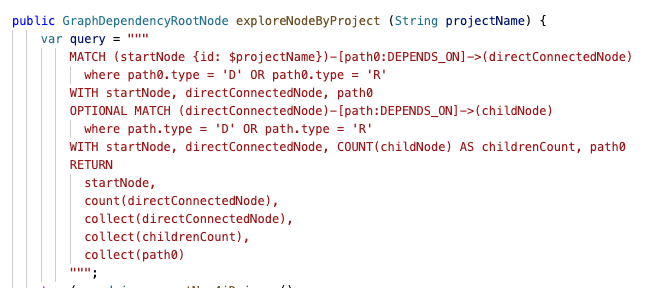
\includegraphics[width=\textwidth]{query-cipher} 
      \caption{Esempio di \textit{query} Cypher per l'esplorazione dell'albero delle dipendenze.}
      \label{fig:query-cipher}
  \end{minipage}\hfill
  \begin{minipage}{0.450\textwidth}
    \centering
    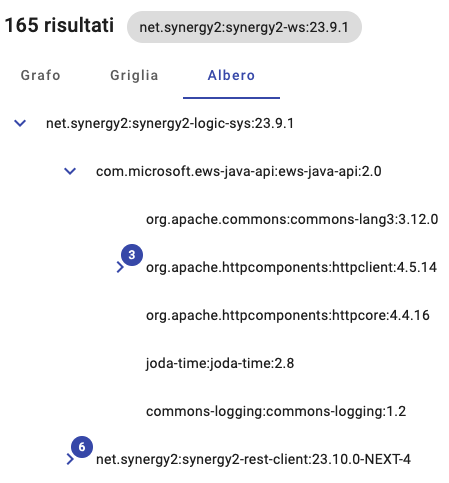
\includegraphics[width=.6\textwidth]{frontend-4}
    \caption{Risultato query \ref*{fig:query-cipher}.}
    \label{fig:frontend-4-bis}
  \end{minipage}
\end{figure}

\subsection*{Ricerca di aggiornamenti e vulnerabilità}
Per la ricerca di aggiornamenti delle dipendenze, ho utilizzato i servizi gratuiti offerti da \textbf{OSS Index},
che permettono di verificare se una dipendenza è aggiornata o meno.\\
Effettuando, ad esempio, la seguente chiamata \textit{GET} \textit{REST} al servizio \\
% use small text inside lstlisting
\begin{lstlisting}[language=Java, caption={Esempio di chiamata al servizio \textbf{OSS Index} per la ricerca di aggiornamenti.},captionpos=b, label={lst:oss-index}
  ,basicstyle=\small]
  https://search.maven.org/solrsearch/select?q=g:com.google.code.gson+a:gson
\end{lstlisting}
avremo come risultato un \textit{JSON} contenente una serie di informazioni riguardanti il pacchetto, tra cui
l'ultima versione disponibile.\\

Questa chiamata viene effettuata per ogni dipendenza del progetto selezionato, e viene confrontata con la versione utilizzata nel progetto.\\
In caso di aggiornamento, viene stampato un messaggio di avviso, come mostrato nella figura \ref{fig:frontend-8}.\\

Per i prossimi sviluppi del progetto, è previsto l'inserimento di questa informazione direttamente nella riga della tabella 
che stiamo visualizzando, in modo da poter identificare in modo più semplice le dipendenze che hanno bisogno di un aggiornamento.\\

Per la ricerca di vulnerabilità, ho utilizzato il servizio \textbf{OWASP Dependency-Check}, che permette di verificare se una dipendenza
ha delle vulnerabilità.\\
Anche in questo caso vengono raccolti i risultati per ogni dipendenza, e in caso di vulnerabilità viene stampato un messaggio di avviso.
\section{Verifica e validazione}
La verifica e la validazione sono due attività fondamentali per garantire la qualità del prodotto software.
Queste attività sono svolte durante tutto il ciclo di vita del software, e sono svolte in parallelo con le attività di sviluppo.
\subsection*{Analisi statica}
Per analisi statica si intende l'analisi del codice sorgente senza eseguirlo, per determinare se il codice sorgente rispetta 
le regole di codifica, le convenzioni adottate e per calcolare alcune metriche di qualità del codice.\\
Per l'analisi statica del codice sorgente Java ho utilizzato IntelliJ IDEA, che
durante la scrittura del codice segnala in tempo reale eventuali errori di sintassi, errori di logica, e segnala anche
se il codice scritto non rispetta alcune convenzioni di codifica imposte dal \textit{team} di sviluppo.\\

Per l'analisi statica del codice sorgente del progetto \textit{client} ho utilizzato WebStorm che, come IntelliJ IDEA,
segnala in tempo reale eventuali errori di sintassi, errori di logica.
In aggiunta, ho utilizzato \textbf{ESLint}, che è un \textit{tool} di analisi statica del codice sorgente JavaScript e
TypeScript, che permette, a prescindere dall'editor utilizzato, di segnalare eventuali errori di sintassi e di controllare
che il codice scritto rispetti le convenzioni di codifica imposte; \\

Un'altro strumento utilizzato, in modo asincrono, per l'analisi statica del codice sorgente è \textbf{SonarQube}, 
un \textit{tool} di analisi statica del codice sorgente, che permette di calcolare alcune metriche di qualità del codice,
e di segnalare eventuali problemi di codifica, e di logica.\\
SonarQube è stato integrato con Jenkins, in modo tale che ad ogni \textit{commit} sul \textit{repository}
del codice sorgente, viene eseguita l'analisi statica del codice sorgente, e vengono segnalati eventuali problemi, mantenendo 
lo storico delle analisi effettuate, evidenziano eventuali miglioramenti o peggioramenti del codice sorgente, come mostrato in 
figura \ref{fig:sonar1} e \ref{fig:sonar2}.\\

\begin{figure}[h]
  \centering
  \begin{minipage}{0.49\textwidth}
      \centering
      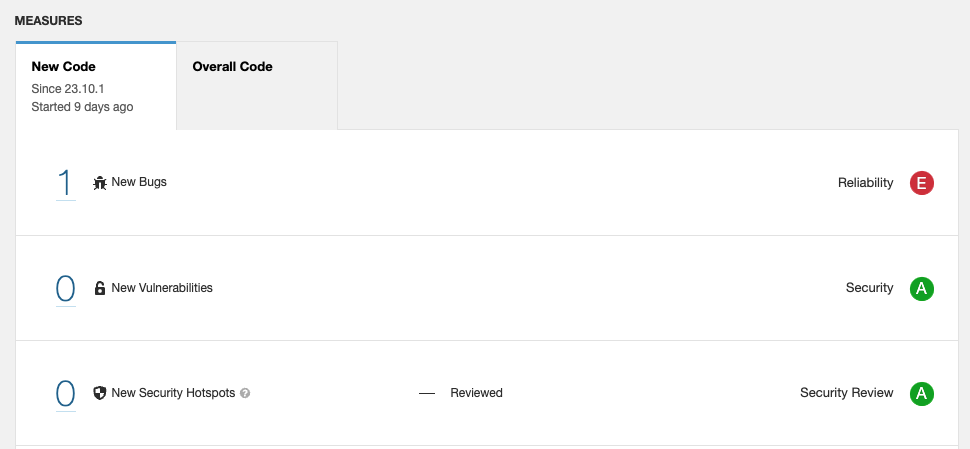
\includegraphics[width=\textwidth]{sonar1} 
      \caption{Dashboard di SonarQube.}
      \label{fig:sonar1}
  \end{minipage}\hfill
  \begin{minipage}{0.49\textwidth}
    \centering
    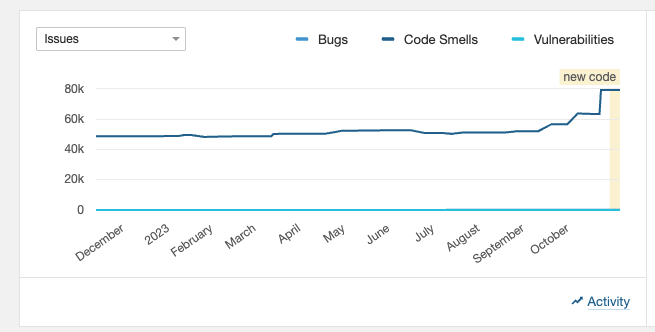
\includegraphics[width=\textwidth]{sonar2}
    \caption{Statistiche di SonarQube.}
    \label{fig:sonar2}
  \end{minipage}
\end{figure}

\subsection*{Analisi dinamica}
L'analisi dinamica è l'analisi del codice sorgente eseguendolo, per determinare se il codice sorgente rispetta
le specifiche e le aspettative.\\
Ho effettuato tre tipi di \textit{test}, i \textit{test} di unità, i \textit{test} di integrazione e i \textit{test} \textit{end-to-end}.\\
\subsubsection*{Test di unità}
I \textit{test} di unità rappresentano una componente fondamentale nello sviluppo del software, 
essenziali per garantire la qualità e l'affidabilità del codice. 
Ho adottato JUnit, un framework popolare per la scrittura di \textit{test} di unità in ambienti Java, 
per validare la correttezza delle singole unità di codice del progetto.

JUnit è stato scelto per la sua ampia adozione nella comunità Java e per la sua integrazione con gli ambienti di sviluppo e i sistemi di build che abbiamo utilizzato. La sua semplicità nell'annotare i metodi di \textit{test} e la possibilità di eseguire \textit{test} in modo ripetibile e automatizzato hanno reso JUnit lo strumento ideale per il nostro progetto.

I \textit{test} di unità sono stati implementati seguendo il principio del \textit{First Testing}: 
prima della scrittura del codice funzionale, sono stati definiti i \textit{test} per validare il comportamento atteso delle varie unità. 
Questo approccio ha contribuito a mantenere un alto standard di qualità del codice e a identificare precocemente eventuali errori.

Per ogni classe principale del progetto, è stata creata una classe di \textit{test} corrispondente. 
I \textit{test} sono stati focalizzati sulle funzionalità critiche, come la gestione delle eccezioni, 
la validazione dei dati in input e l'accuratezza dei risultati restituiti.

I \textit{test} di unità sono stati integrati nel sistema di build automatizzato, utilizzando Gradle. 
Questo ha permesso di eseguire i \textit{test} automaticamente ad ogni build, 
garantendo che eventuali regressioni o nuovi errori venissero identificati tempestivamente.

L'adozione di JUnit e l'implementazione sistematica di \textit{test} di unità hanno avuto un impatto significativo sulla qualità del software prodotto. 
I \textit{test} hanno aiutato a mantenere il codice robusto e flessibile, facilitando anche le fasi di \textit{refactoring} e l'aggiunta di nuove funzionalità. 
Inoltre, l'approccio di test-driven development ha migliorato la mia capacità di scrivere codice più chiaro e mantenibile.

\subsubsection{\textit{Test-driven development}}
Il \textit{\gls{tdd}} è una metodologia di sviluppo software che inverte l'ordine tradizionale dello sviluppo. 
Invece di scrivere prima il codice e poi i \textit{test} per verificare che il codice funzioni come previsto, nel TDD si scrivono prima 
i \textit{test} e poi il codice che deve superarli. Ecco i passaggi chiave del TDD:
\begin{enumerate}
  \item \textbf{Scrivere un test}: Prima di scrivere il codice funzionale, si scrive un \textit{test} per una nuova funzionalità. Questo \textit{test} fallirà inizialmente, poiché la funzionalità non è stata ancora implementata.
  \item \textbf{Scrivere il codice minimo necessario}: Si scrive poi il codice necessario affinché il \textit{test} passi. Questo codice non deve essere perfetto; l'obiettivo è semplicemente far passare il \textit{test} 
  \item \textit{\textbf{Refactoring}}: Una volta che il \textit{test} è superato, si procede con il \textit{refactoring} del codice. Questo passaggio consiste nel migliorare e pulire il codice senza modificarne la funzionalità, assicurandosi che i \textit{test} continuino a passare.
  \item \textbf{Ripetizione}: Questo ciclo viene ripetuto per ogni nuova funzionalità o miglioramento. Si scrive un test, si fa in modo che passi, e poi si rifinisce il codice.
\end{enumerate}

I benefici del TDD includono:
\begin{itemize}
  \item \textbf{Migliore \textit{design} del codice}: Poiché si scrive il \textit{test} prima del codice, si è spinti a pensare più attentamente a come il codice dovrebbe funzionare e alla sua interfaccia pubblica.
  \item \textbf{Codice più affidabile}: Poiché si scrive un \textit{test} per ogni nuova funzionalità, si ha una copertura di \textit{test} più ampia, il che aiuta a identificare e correggere gli errori più rapidamente.
  \item \textbf{Facilità di \textit{refactoring}}: Avendo una suite di \textit{test} che copre il codice, si può fare \textit{refactoring} con maggiore sicurezza, sapendo che i \textit{test} rileveranno eventuali regressioni introdotte.
\end{itemize}

Tuttavia, il TDD richiede disciplina e può richiedere più tempo all'inizio, 
specialmente per chi non è abituato a questa metodologia. 
Ma nel lungo termine, può portare a un codice più pulito, più facile da mantenere e con meno \textit{bug}.

\subsubsection{Test di unità per il \textit{frontend}}
Nel \textit{frontend} Angular, per la scrittura dei \textit{test} di unità mi sono affidato a \textit{Jest}, 
un \textit{framework} di testing JavaScript.
\textbf{Jest} è stato scelto per la sua ampia adozione nella comunità JavaScript 
e per la sua integrazione con gli ambienti di sviluppo e i sistemi di build che abbiamo utilizzato. 

\subsubsection*{Test di integrazione}
I \textit{test} di integrazione sono stati implementati per verificare il corretto funzionamento 
delle interazioni tra le varie componenti del sistema.
Per farlo ho utilizzato ancora JUnit, riuscendo a configurarlo in modo tale che
i \textit{test} di integrazione vengano eseguiti solo quando necessario, 
e non ad ogni \textit{build} del progetto, come invece avviene per i \textit{test} di unità.\\

Con i \textit{test} di integrazione ho verificato che tutti i servizi esposti dal \textit{backend} funzionassero correttamente,
e che il \textit{client} riuscisse a comunicare correttamente.
Nel caso dei test, il \textit{client} è stato simulato utilizzando delle chiamate \textit{HTTP} 
direttamente da codice Java, senza utilizzare il \textit{client} Angular.\\
Questo ci ha permesso di verificare che il \textit{backend} funzionasse correttamente,
senza dover dipendere dal \textit{client} Angular.

\subsubsection*{Test \textit{End-to-End}}
I \textit{test} \textit{end-to-end} sono stati l'ultimo tassello per garantire la qualità del prodotto.
Ho utilizzato \textbf{Playwright}, una libreria \textbf{Node.js} per l'automazione dei \textit{test} \textit{end-to-end}
 per applicazioni \textit{web}, sviluppata da \textbf{Microsoft}.\\
Playwright è stato scelto per la sua ampia adozione nella comunità di \azienda{},
e perchè non prevede nessun piano di abbonamento, a differenza di tanti altri.

L'obiettivo dei \textit{test} \textit{end-to-end} è quello di simulare l'interazione di 
un utente con il sistema, e verificare che il sistema funzioni correttamente.\\
Un prerequisito per l'esecuzione dei \textit{test} \textit{end-to-end} è che il sistema sia in esecuzione
e che il \textit{server} \textit{web} sia raggiungibile.\\
Per questo motivo, i \textit{test} \textit{end-to-end} sono stati eseguiti in un ambiente di \textit{staging},
in modo tale da poter simulare l'interazione di un utente con il sistema, senza dover dipendere
dall'ambiente di produzione.\\

Durante l'esecuzione dei \textit{test} \textit{end-to-end} è possibile abilitare la modalità \textit{debug},
in modo tale da poter visualizzare l'esecuzione dei \textit{test} in tempo reale, e poter intervenire
in caso di errori o sospendere l'esecuzione per analizzare lo stato del sistema.\\

In caso di errori, Playwright permette di catturare uno \textit{screenshot} della pagina,
in modo tale da poter analizzare l'errore e capire la causa anche in un secondo momento.\\

